
\subsection{Azure Trace Simulations}

\paragraph{Methodology.} Trace is big. We sample the trace based on the distribution of the functions size and popularities in the full day's trace. The resulting traces are smaller and more tractable for evaluating the Performance of a single server. Also allows us to use different trace subsets with different characteristics to allow for a more generalized evaluation. 

Metrics: 
\begin{itemize}
\item Cold start \% 
\item \% Latency increase due to cold starts
\item Requests dropped 
\end{itemize}

2 graphs per trace, and 2 traces = 4 graphs. 

\textbf{Outcome:} Caching based approaches reduce cold starts by 50\% . For heavier traces, the effect is even more pronounced. 


\subsection{OpenWhisk Benchmarks}

\subsubsection{Micro traces}. Just like microbenchmarks, we generate workload traces that are vary one characteristic at a time to allow us to understand the effectiveness of our keep-alive policies in isolation.

Iat: the inter-arrival time is varied, rest  are constant.

We use lookbusy to generate load inside each function.

Metrics:
\begin{itemize}
\item Cold start \%
\item System Utilization (Low priority) 
\item Requests Dropped (Low priority)
\end{itemize}

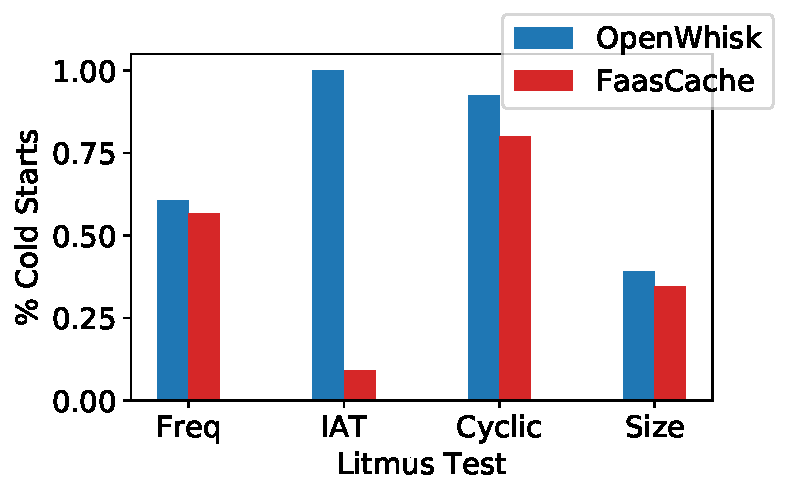
\includegraphics[width=0.4\textwidth]{../graphs/litmus_2.pdf}

\textbf{Outcome:} GD can reduce cold start rate by 50\% in many cases. It also reduces the number of requests dropped by OpenWhisk. \emph{The system utilization (CPU) should come here.}


\subsubsection{Real Applications.}

For TensorFlow, numpy, etc., what is the impact on their latency?

\subsection{Provisioning}

\begin{figure}[t]
  \centering
  \includegraphics[width=0.48\textwidth]{../graphs/dyn-scale-392.pdf}  
  \caption{Dyn scaling}
  \label{fig:dyn-scale}
\end{figure}


\textbf{Outcome:} Dynamic scaling allows us to reduce memory usage by adjusting to hit-rate. 


\subsection{Trace Analysis.}

Reuse distance vs. time heatmap? 